%!TEX root = ../chapter06.tex 
%----------------------------------------------------------------------------------------
%	
%---------------------------------------------------------------------------------------- 
%----------------------------------------------------------------------------------------
%	 
%----------------------------------------------------------------------------------------


\newpage 
\loadgeometry{marginlayout}  
\pagestyle{scrheadings} % Print headers again  
\KOMAoptions{
	headwidth=textwithmarginpar,
	headsepline=true,
	headsepline= 0.5pt,
	footwidth=textwithmarginpar,
}   
\onehalfspacing    
\section{Égalité de vecteurs}
$B$ est l'image de $A$ par la translation $t$ de vecteur $\vv{XY}$. 
\begin{figure}[hb]   
	\begin{tikzpicture}[scale=0.80]
		\tkzInit[xmin=-2, xmax=12,ymax=5]
		\tkzSetUpPoint[size=3, fill=black]
		\tkzfctset{tan style/.style={->,>=latex, color=red, line width=1.2pt}}   
		\tkzSetUpLine[line width= 1.2pt, add=.2 and .2]  
		\begin{scope}[dashed] 
			%			\tkzGrid[sub, subxstep=1, subystep=0.5]
			\tkzGrid[xstep=1,ystep=1]
		\end{scope} 
		\tkzDefPoint(3,2.0){X}
		\tkzDefShiftPoint[X](4,1.5){Y}
		\tkzDrawSegments[->,>=latex](X,Y)
		%		\tkzLabelSegment[above,font=\scriptsize](U,V){$\vv{u}$} 
		%		\tkzDefPoint(2,.5){A}
		%		\tkzDefPointWith[colinear=at A](U,V)\tkzGetPoint{A'}
		%		\tkzDrawSegments[->,>=latex](A,A')
		%		\tkzDefPoint(0,1.0){B}
		\tkzDefPoint(8,1.5){C}
		\tkzDefPoint(0,3.0){A}
		\tkzDrawPoints[shape=cross out](A,C)
		\tkzLabelPoints(A,C,X,Y)
	\end{tikzpicture} 
	\caption{$B$ est l'image de $A$ par la translation $\protect\vv{XY}$ \\
		$C$ a la même image par les translations $\protect\vv{XY}$ et celle de vecteur $\protect\vv{AB}$ (la démonstration nécessite le theorème \ref{chapitre06:theorem:parallelogrammetransitif}).\\
		$\protect\vv{XY}$ et $\protect\vv{AB}$ représentent la même translation nommée vecteur $\protect\vv{u}$.  \\
		On écrit $\protect\vv{u}=\protect\vv{AB}=\protect\vv{XY}$.
	}
\end{figure}  
On dira que les vecteurs $\vv{AB}$,  et $\vv{XY}$ sont des représentants \xout{de la translation $t$} du vecteur $\vv{XY}$\sidenote{\og Vecteur $\vv{XY}$ \fg{} et \og la translation de vecteur $\vv{XY}$ \fg{} signifient désormais la même chose.}. On désigne par $\vv{u}$ cette translation et on écrit :
\setlength{\belowdisplayskip}{0pt}
\[
\vv{u}=\vv{AA'}=\vv{BB'}=\vv{XY}
\]   
\begin{definition}[Dans un repère $(O;I,J)$] deux vecteurs sont égaux $\vv{AB}=\vv{CD}$ s.s.i. leurs couples de coordonnées sont égaux. 
\end{definition}  
\begin{postulat}  L'égalité de vecteurs reste vraie si on change de repère et :
	
	$\vv{AB}=\vv{CD}$  si et seulement si $AB\textbf{D}C$ est un parallélogramme. 
\end{postulat}  
\vfill 



\begin{definition}[caractéristiques d'un vecteur $\vv{u}\neq \vv{0}$] Soit le vecteur $\vv{u}$ et ses représentants $\vv{AB}$  $\vv{XY}$. 
	
	Le vecteur $\vv{u}$ et tous ses représentants sont caractérisés par :
	\begin{description}
		\item[une même \textbf{direction}]\sidenote{On ne dit pas que deux vecteurs sont parallèles. \\
			On ne dit pas qu'un vecteur est parallèle à une droite.} parallèle à la droite $\left( {AA'} \right)\mathbin{\!/\mkern-2mu/\!}  \left( {XY} \right)$.
		\item[un même \textbf{sens}] selon la flèche, de $A$ vers $B$, de $X$ vers $Y$.
		\item[une même \textbf{norme}] notée $\left\| \vv{u} \right\|= AB=XY$.
	\end{description}  
\end{definition} 


\begin{definition}[ Vecteur nul $\vv{0}$] est la translation identité  
	$ \vv{0}=\vv{AA}=\vv{BB}=\vv{CC}=\ldots$ Sa norme vaut $\norm{\vv{0}}=0$.\sidenote{Le vecteur $\vv{0}$ n'a ni direction ni sens !}
\end{definition}   

%----------------------------------------------------------------------------------------
%	 
%----------------------------------------------------------------------------------------
\newpage  
\subsection{Coordonnées du milieu d'un segment}
\begin{tBox}
	$\vv{AM}=\vv{MB}$ si et seulement si $M$ est le milieu du segment $[AB]$ 
\end{tBox} 

\begin{marginfigure}
	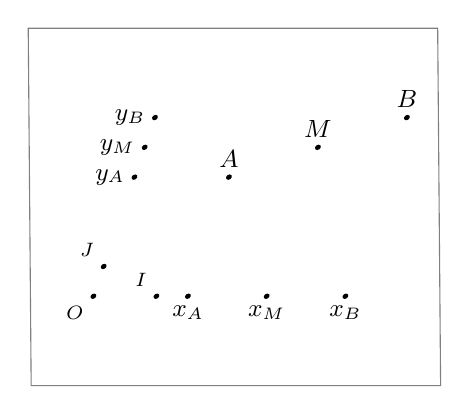
\begin{tikzpicture}[scale=0.40]
		\tkzInit[xmin=-8,xmax=10,ymin=-7,ymax=8  ]
		\pgftransformcm{1}{0}{sin(19)}{cos(19)}{\pgfpointorigin}
		\path[clip,preaction = {draw=gray}] 
		(+12,-3) -- (-1,-3) -- (-5,9) -- (8,9) -- cycle;
		%\tkzGrid[color=gray](-9,-7)(11,7)
		\tkzDrawXY[ noticks, line width=1pt] 
		\filldraw 
		(0,0) circle (2pt) node[align=left, below left] {\scriptsize $O$} ;
		\filldraw 
		(2,0) circle (2pt) node[align=left, above left] {\scriptsize $I$} ;
		\filldraw 
		(0,1) circle (2pt) node[align=left, above left] {\scriptsize$J$} ;
		\filldraw 
		(3,4) circle (2pt) node[align=left, above] {\small$A$} ;
		\filldraw 
		(3,0) circle (2pt) node[align=left, below] {\small$x_A$} ;
		\filldraw 
		(0,4) circle (2pt) node[align=left, left] {\small$y_A$} ;
		\filldraw  
		(8,6) circle (2pt) node[align=left, above] {\small$B$} ;
		\filldraw 
		(8,0) circle (2pt) node[align=left, below] {\small$x_B$} ;
		\filldraw 
		(0,6) circle (2pt) node[align=left, left] {\small$y_B$} ;
		\filldraw  
		(5.5,5) circle (2pt) node[align=left, above] {\small$M$} ;
		\filldraw 
		(5.5,0) circle (2pt) node[align=left, below] {\small$x_M$} ;
		\filldraw 
		(0,5) circle (2pt) node[align=left, left] {\small$y_M$} ;
		\filldraw 	;		
		\tkzDefPoint(5.5, 5){M};
		\tkzDefPoint(5.5,0){xM};
		\tkzDefPoint(0, 5){yM};
		\tkzDrawSegments[dashed](M,xM M,yM);
		\tkzDefPoint(3,4){A};
		\tkzDefPoint(3,0){xA};
		\tkzDefPoint(0,4){yA};
		\tkzDrawSegments[dashed](A,xA A,yA);
		\tkzDefPoint(8,6){B};
		\tkzDefPoint(8,0){xB};
		\tkzDefPoint(0,6){yB};
		\tkzDrawSegments[dashed](B,xB B,yB);
		\tkzDrawSegments[line width=2pt](A,M M,B);
		\tkzMarkSegments[mark=s||](A,M M,B);
		\tkzMarkSegments[mark=|||](xA,xM xM,xB);
		\tkzMarkSegments[mark=s|](yA,yM yM,yB);
	\end{tikzpicture}  
\end{marginfigure} 
\begin{proof}[Démonstration]\hfill 
	\begin{align*}
		&\text{$M$ est le milieu de $[AB]$} \\
		& \iff \vv{AM}=\vv{MB} \\
		& \iff \vv{AM}\begin{pmatrix}
			x_M-x_A \\ y_M-y_A
		\end{pmatrix}=\vv{MB}\begin{pmatrix}
			x_B-x_M\\ y_B-y_M
		\end{pmatrix} \\
		& \iff \begin{cases}
			x_M-x_A = x_B-x_M  \\  y_M-y_A = y_B-y_M
		\end{cases} 
		\iff \begin{cases}
			2x_M = x_A + x_B  \\ 2y_M = y_A + y_B
		\end{cases} \\
		& \iff \begin{cases}
			x_M =\frac{x_A+x_B}{2} \\ y_M =\frac{y_A+y_B}{2}
		\end{cases}  
	\end{align*} 
	%	\vfill 
\end{proof} 
\begin{theorem}[formule pour les coordonnées du milieu d'un segment]
	Soit $A(x_A;y_A)$ et $B(x_B;y_B)$ dans un repère.
	
	Le milieu $M(x_M;y_M)$ de $[AB]$ est le point de coordonnées :
	\begin{align*}
		x_M&=\frac{x_A+x_B}{2}\\
		y_M&=\frac{y_A+y_B}{2}
	\end{align*}
\end{theorem} 


\begin{example}
	On considère les points $A(1~;~2)$, $B(3~;~1,5)$, $C(4~;~0,5)$ et $D(2~;~1)$.  
	Montrer que le quadrilatère $ABCD$ est un parallélogramme en déterminant les coordonnées des milieux des diagonales.
\end{example}
\vfill 


%----------------------------------------------------------------------------------------
%	 
%----------------------------------------------------------------------------------------
